\documentclass[border=10pt]{standalone}
\usepackage{tikz}
\usetikzlibrary{positioning}
\begin{document}
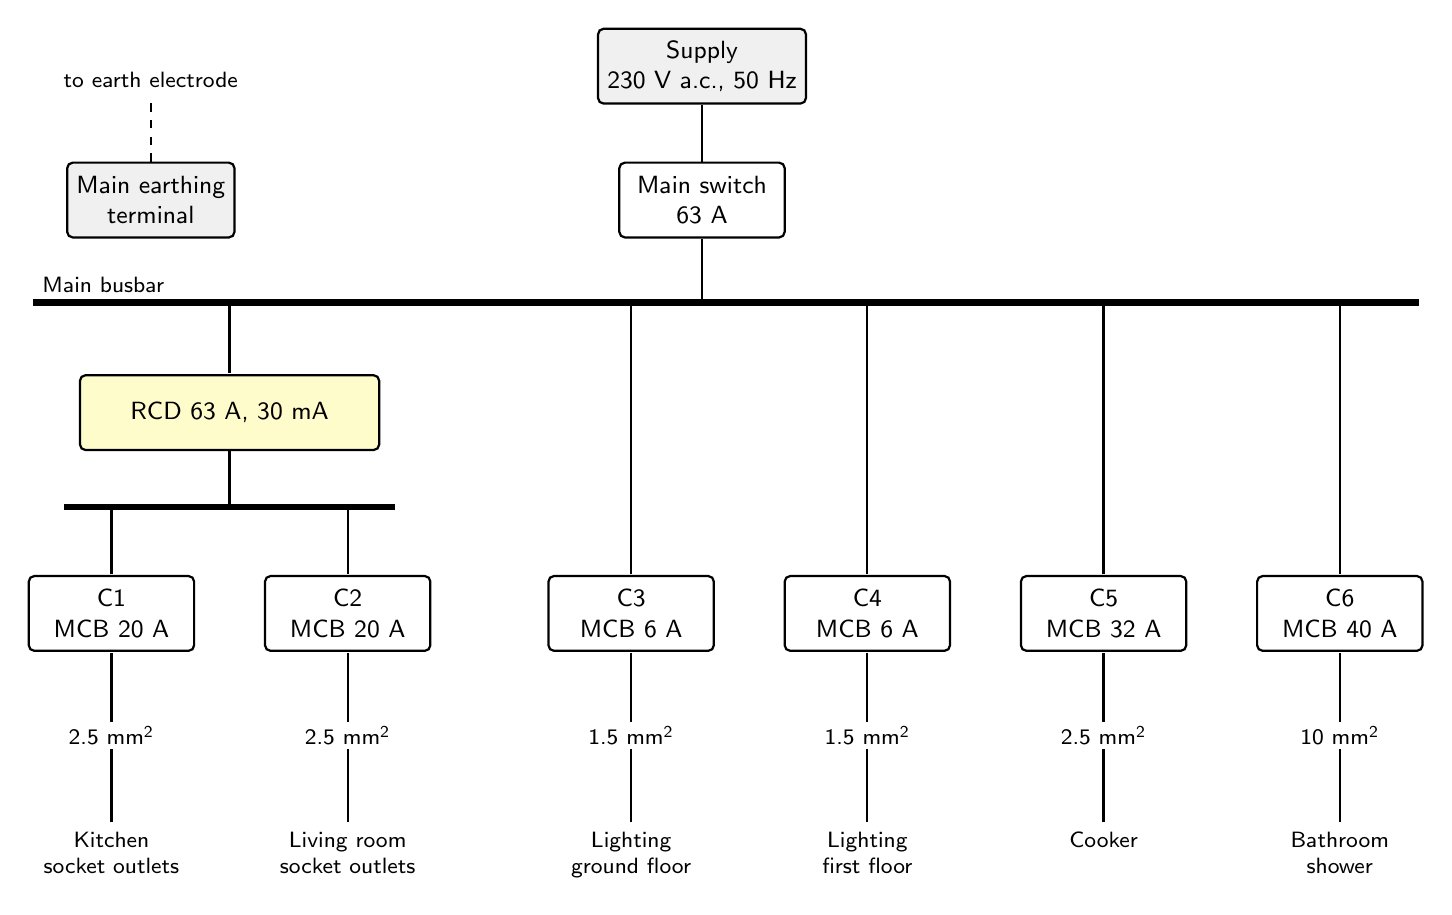
\begin{tikzpicture}[
  font=\sffamily\small,
  dev/.style={draw, thick, rounded corners=2pt, minimum width=2.1cm, minimum height=0.95cm,
              align=center, fill=white},
  wire/.style={thick},
  bus/.style={line width=2.4pt},
  cable/.style={font=\sffamily\footnotesize, fill=white, inner sep=1.5pt},
  load/.style={align=center, font=\sffamily\footnotesize}
]
  \node[dev, fill=gray!12] (sup) at (2.5,0) {Supply\\230 V a.c., 50 Hz};
  \node[dev] (main) at (2.5,-1.7) {Main switch\\63 A};
  \node[dev, fill=gray!12] (met) at (-4.5,-1.7) {Main earthing\\terminal};
  \draw[wire] (sup) -- (main);
  \draw[wire] (main) -- (2.5,-3);
  \draw[wire, dashed] (met) -- (-4.5,-0.4) node[above, font=\sffamily\footnotesize] {to earth electrode};

  \draw[bus] (-6,-3) -- (11.6,-3);
  \node[font=\sffamily\footnotesize, anchor=south west] at (-6,-3) {Main busbar};

  \draw[wire] (-3.5,-3) -- (-3.5,-3.9);
  \node[dev, fill=yellow!20, minimum width=3.8cm] (rcd) at (-3.5,-4.4) {RCD 63 A, 30 mA};
  \draw[wire] (rcd) -- (-3.5,-5.6);
  \draw[bus] (-5.6,-5.6) -- (-1.4,-5.6);

  \draw[wire] (-5,-5.6) -- (-5,-6.45);
  \node[dev] (c1) at (-5,-6.95) {C1\\MCB 20 A};
  \draw[wire] (-2,-5.6) -- (-2,-6.45);
  \node[dev] (c2) at (-2,-6.95) {C2\\MCB 20 A};

  \foreach \x/\id/\mcb in {1.6/C3/6, 4.6/C4/6, 7.6/C5/32, 10.6/C6/40} {
    \draw[wire] (\x,-3) -- (\x,-6.45);
    \node[dev] at (\x,-6.95) {\id\\MCB \mcb\ A};
  }

  \foreach \x/\size/\label in {
      -5/2.5/{Kitchen\\socket outlets},
      -2/2.5/{Living room\\socket outlets},
      1.6/1.5/{Lighting\\ground floor},
      4.6/1.5/{Lighting\\first floor},
      7.6/2.5/{Cooker},
      10.6/10/{Bathroom\\shower}} {
    \draw[wire] (\x,-7.45) -- (\x,-9.6);
    \node[cable] at (\x,-8.5) {\size\ mm\textsuperscript{2}};
    \node[load, below] at (\x,-9.6) {\label};
  }
\end{tikzpicture}
\end{document}
